\documentclass[a4paper,11pt]{article}
\usepackage[scale=0.85]{geometry}
\usepackage{titling}
\usepackage{amsmath,amsfonts}
\usepackage{xcolor}
\usepackage{braket}
\usepackage{bm}
\usepackage{tensor}
\usepackage{cleveref}
% \usepackage{MnSymbol}
\usepackage{mhchem}
\usepackage{graphicx}
\usepackage{cite}
\usepackage{booktabs}
\usepackage{wrapfig}
\usepackage{bbm}
\usepackage{framed}
\usepackage{frame}
\usepackage[shortlabels]{enumitem}
\title{Homework for Week 14}
\author{Chen Xue  2022311901}
\begin{document}
\maketitle

\section{Kramers-Wannier Duality on the Boundary}
Defining $s = e^{i\theta_v}$, $\theta_v \in \{0, \pi\}$, then $ e^{i ({\rm d}\theta)_l} = s_v s_{v+1}$, where $({\rm d}\theta)_l = \theta_{v+1} - \theta_v$. With smooth boundary, we know that $s_{(x, 1)} s_{(x,0)} \equiv 0$, which means we know $({\rm d}\theta)_l$, just like the given derivative on the boundary in continuum. While the rough boundary condition specifies $\theta_{(x,0)} = 0$ just like Dirichlet boundary condition.\\
In low temperature expansion, the domain walls form closed loop in dual lattice without touching boundary. When it touches the boundary, if boundary is smooth, it does not need to be closed, the endpoints can locate outside the macroscopic boundary; On the other hand, if the boundary is rough, domain walls still need to be closed loop.\\
In high temperature expansion, only current loop contributes to the path integral when the boundary is smooth; But when boundary is rough, the endpoints can locate at $(x,0)$. 
\begin{figure} [h]
    \centering
    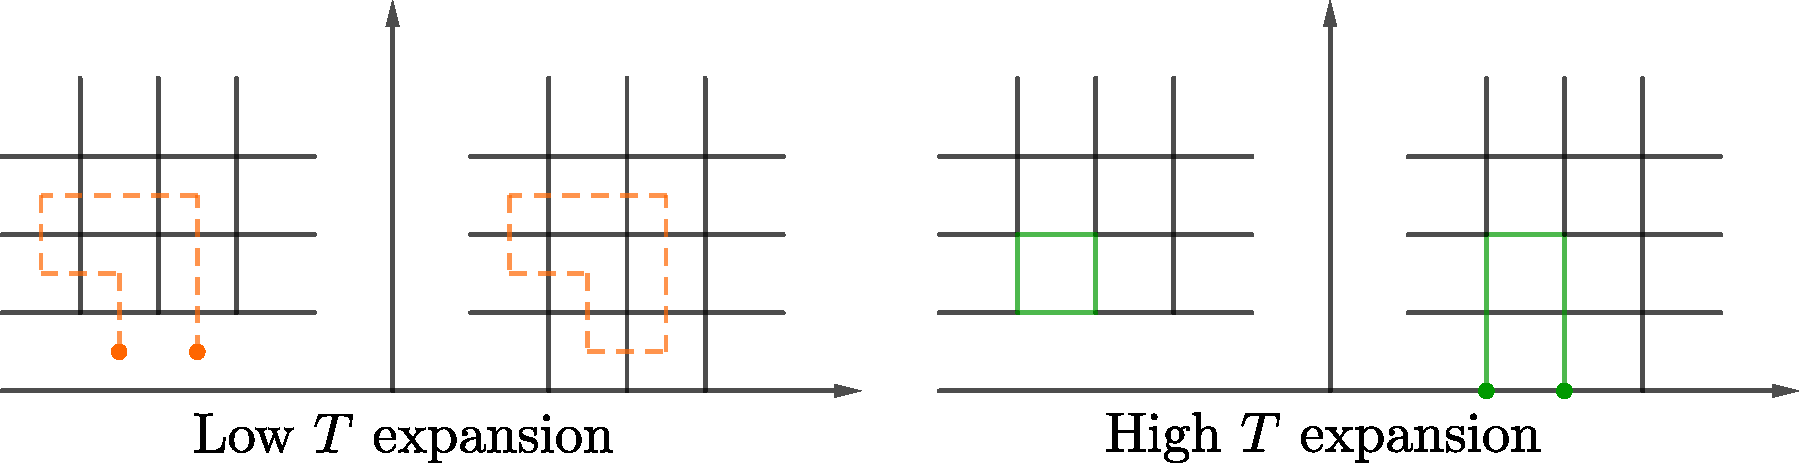
\includegraphics[width = \linewidth]{boundary.pdf}
\end{figure}
Under Kramers-Wannier duality, Neumann boundary condition $\longleftrightarrow $ Dirichlet boundary condition.\\
The sum over current loop configurations in path integral in low $T$ expansion dual to sum over domain configurations in high $T'$ expansion but with a factor $\frac{1}{2}$. This is because one domain wall configuration corresponding to two domain configuration. But when the dual side has a Dirichlet boundary, half of the configurations are excluded. So one domain configuration corresponding to one current loop in the original side.

\section{Kramers-Wannier Duality in (1+1)D quantum Ising Model}
\paragraph{}









\end{document}